\documentclass[twocolumn,preprintnumbers,amsmath,amssymb]{revtex4}
\usepackage{graphicx}% Include figure files
\usepackage{dcolumn}% Align table columns on decimal point
\usepackage{bm}% bold math
\usepackage{units}
\usepackage{braket}
\usepackage{soul}
\usepackage[spanish]{babel} %para español
%este paquete permite usar los acentos normales
% es decir á en lugar de \'a
\usepackage[utf8]{inputenc} 


\makeatletter
\newenvironment{figurehere}
{\def\@captype{figure}}
{}
\makeatother

\begin{document}

\title{Propiedades e interpretación del taquión}
\author{Brayan Alexander Muñoz B.\footnote{\href{mailto:restrepo@udea.edu.co}{balexander.munoz@udea.edu.co}}}

\affiliation{Instituto de Física, Facultad de Ciencias Exactas y Naturales, Universidad de Antioquia UdeA, Calle 70 No. 52-21, Medellín, Colombia}

\date{\today}

\begin{abstract}

Los taquiones son partículas hipotéticas que viajan más rápido que la luz. Se les atribuyen propiedades inexplicables el día de hoy como lo es su masa compleja. La mayoría de los físicos creen que este tipo de partículas más rápidas que la luz no pueden existir, pues no son consistentes con las leyes conocidas del universo tales como la causalidad  \cite{Randall:900484}. Más que eso, en 1967 se propuso que las partículas taquiónicas podrían ser elementos de un campo cuántico con masa imaginaria. Algunas partículas como los bosones o los inflatones pueden presentar estados taquiónicos como los del campo en un punto altamente inestable. Ya que dichos campos son inestables, se crean condensados taquiónicos que dispersan una gran cantidad de particulas \cite{eberly2013review}. No se ha encontrado evidencia experimental de la existencia de tales partículas, sin embargo en este artículo se cuestionan sus interpretaciones conceptuales así como sus propiedades y consecuencias como campo y como partícula.

\bigskip	
\noindent
Palabras clave: Taquión, campo, partículas, luz, causalidad, causalidad, bosones, inflatones, condensado taquiónico.

\end{abstract}

\maketitle

\section{Introducción}

Por mucho tiempo se ha pensado que ninguna partícula puede viajar a velocidades superiores a la de la luz en el vacío, y esta limitación es una consecuencia directa de la relatividad general de Einstein \cite{hill2012einstein}. Sin embargo, hay investigadores que afirman que no existe inconsistencia alguna entre partículas con dicha velocidad y la relatividad \cite{bilaniuk1969particles}. E. C. G. Sudarshan, V.K Deshpande y Baidyanath Misra fueron los primeros en proponer la existencia de partículas más rápidas que la luz y las llamaron "meta partículas". Después de eso, Robert Ehrlich y Arnold Sommerfeld también propusieron la posibilidad de que las partículas se movieran más rápido que la luz. El término "taquión" se acuñó por primera vez en el artículo de Gerald Feinberg de 1967 \cite{feinberg1967possibility} y aquí se propuso que las partículas taquiónicas podrían ser cuantos de un campo cuántico con masa imaginaria. Sin embargo, pronto se dio cuenta de que las excitaciones de tales campos de masas imaginarios no se propagan bajo ninguna circunstancia más rápido que la luz, y en cambio la masa imaginaria da lugar a una inestabilidad conocida como condensación de taquiones. Así, en la física moderna, el término taquión se refiere a menudo a campos de masa imaginarios en lugar de a partículas más rápidas que la luz. Estos campos de masa han llegado a desempeñar un papel importante en la física moderna en áreas como la teoría de cuerdas, teoría M y cosmología \cite{Randall:900484}.

Por otro lado, la invariancia de Lorentz, el ingrediente principal de la relatividad especial, es uno de los pilares de la física moderna. Aunque la relatividad especial ha sido reemplazada por la relatividad general, la invariancia de Lorentz sigue siendo válida localmente. Todos los campos físicos deben obedecer las leyes de la invariancia de Lorentz local así  como formar un conjunto completo.


En el presente artículo se revisan los conceptos de taquión como partícula y como campo, además de sus propiedades, la masa imaginaria, la reducción de energía al aumentar la velocidad hasta su propia aniquilación y las implicaciones de causalidad. Se cuestiona la hipótesis de campo taquiónico por no formar un conjunto completo de soluciones y no ser un invariante de Lorentz. Además, se aclara la naturaleza inestable de dicho campo y su implicación directa como lo es la condensación taquiónica.

\section{Taquiones como partículas}

En los trabajos de Einstein se evidencia cómo a medida que una partícula se acerca a la velocidad de la luz, su masa tiende a aumentar infinitamente. Esto se evidencia desde la ecuación:

\begin{equation}
E = \frac{mc^2}{\sqrt{1-v^2/c^2}}.
\label{eq:Emc}
\end{equation}

Sin embargo no todas las partículas rápidas se producen acelerándose, tomemos los fotones o los neutrinos.
Es decir, la velocidad límite y el aumento de masa solo se cumple para partículas masivas.

Consideremos una partícula con energía $E$ y momento $P$. Tomando un marco de referencia donde la partícula se mueve solo en $x$, sin pérdida de generalidad esta debe obedecer la relación:
%
\begin{equation}
E - P_{x}^2 = m_0^2 c^4,
\label{eq:EP}
\end{equation}
%
donde $m_0$ es la masa en reposo. Esta es la ecuación de una hipérbola en $P_x$ y $E$, y  ya que la velocidad viene dada por 
\begin{equation}
v_x = dE/dP_x.
\label{eq:Pendiente}
\end{equation}
Notamos que como esta pendiente es cada vez más pequeña que $c$, incluso eligiendo un marco en el que la energía es increíblemente grande, su velocidad aún no excederá el valor de $c$. Estas partículas masivas las llamaremos de tipo 1.  Aunque la relatividad excluye la aceleración de partículas de tipo 1 a velocidades mayores o iguales que $c$, las partículas tipo 2 serán, como mencionamos anteriormente, las carentes de masa como el fotón o los neutrinos.

Ya que tenemos partículas que viajan siempre más bajo que la velocidad de la luz (clase 1) y partículas que viajan siempre a la velocidad de la luz (clase 2) ¿no es posible que un nuevo tipo (clase 3) de partícula que tiene una velocidad mayor que $c$ se emita durante algún proceso aún no descubierto?
 
 Pues bien, en la ecuación \eqref{eq:Emc} para que la energía sea un número real, la masa también debe serlo, así que si definimos formalmente la masa del taquión como 
 \begin{equation}
 M_t = im ,
 \label{eq:Mt}
 \end{equation}
 obtenemos la ecuación 
 \begin{equation}
E = \pm \frac{M_t c^2}{\sqrt{v^2/c^2 - 1}} ,
\label{eq:Emtc}
\end{equation}
%
donde notamos que para que la raíz sea real, $v>c$, es decir, la velocidad de la partícula debe ser mayor que la velocidad de la luz. El valor absoluto de estas partículas es llamado meta-masa. Como la masa propia $m_0^2$ se vuelve $-M_t^2$ la ecuación \eqref{eq:EP} queda expresada con un signo menos. Ahora en esta nueva ecuación, la pendiente \eqref{eq:Pendiente} es mayor a $c$ en todas partes y nunca será menor.

\begin{figure}[htb!]
\centering
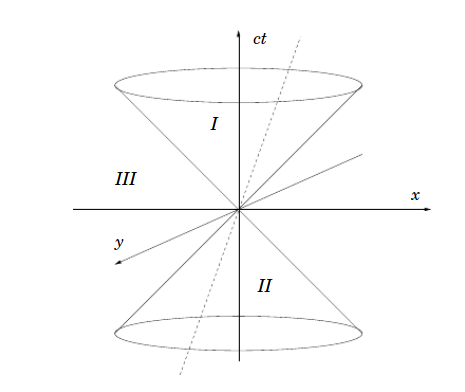
\includegraphics[width=0.9\columnwidth]{conodeluz2.png}
\caption{ Diagrama espacio-temporal o cono de luz donde la luz viaja en trayectorias de $45^{\circ}$ la zona 1 corresponde a trayectorias de partículas de clase 1, las partículas de la clase 2 se mueven sobre el cono de luz, y las partículas clase 3 se mueven en la zona 3. La zona 2 es el pasado.}
\label{fig:cono}
\end{figure}

Cada que la partícula pierde energía, su velocidad aumenta, y si suponemos una partícula cargada eléctricamente, esto implica un efecto de radiación de Cherenkov tal como lo hacen las partículas cargadas ordinarias cuando exceden la velocidad de la luz en un medio. Pero como reducir la energía de un taquión aumenta su velocidad, la partícula irá acelerando cada vez más hasta que su energía sea cero y esta desaparezca, siendo aniquilada por ella misma (su antiparticula).


Todo lo mencionado anteriormente es fuertemente criticado por la comunidad científica, ya que al viajar por una trayectoria en la zona 3 (ver figura \ref{fig:cono}) siempre se puede hallar un sistema de referencia en el cuál la partícula tiene energía positiva pero va hacia atrás en el tiempo.
A pesar de que los taquiones no se han detectado nunca, se pueden detectar estados taquiónicos altamente inestables. Por ejemplo, el bosón de Higgs a alta temperatura fuera de su punto de equilibrio tendría una masa $m^2 <0$, es decir una masa imaginaria y se comporta como un taquión, pero al tender a su punto de más baja energía, se acelera rápidamente y decae. Esto mismo ocurre con el inflatón \cite{nanni2018particle,kostelecky1988static,mazumdar2001assisted}.

\section{Campos de masa imaginarios}

Aquí se estudian las soluciones a la ecuación de Klein-Gordon para un campo escalar $\psi(x)$ con una masa imaginaria como en la ecuación \eqref{eq:Mt}. El desarrollo se limita a los campos escalares porque no hay una representación finita-dimensional del grupo de Lorentz para campos con masa compleja \cite{feinberg1967possibility}.

Partimos de la ecuación en unidades naturales:

\begin{equation}
-\partial _{t}^{2}\psi +\nabla ^{2}\psi =m^{2}\psi,
\label{eq:Klein1}
\end{equation}
que con una masa negativa quedaría de la forma
\begin{equation}
(\nabla^{2} - \partial _{t}^{2} + m_t^{2} ) \psi = 0,
\label{eq:Klein2}
\end{equation}
y tiene como soluciones 

\begin{equation}
\psi_{\pm} = \frac{1}{ (2 \pi)^{3/2} } e^{\pm i \mathbf{k} \mathbf{x}}
\label{eq:KleinSolutions}
\end{equation}

Aquí tanto $k$ como $x$ son cuadrivectores tales que

\begin{equation}
\mathbf{k} = \left(\omega, \vec{\mathbf{k}} \right) , \mathbf{x} = \left(t, \vec{\mathbf{x}} \right)
\label{eq:WK}
\end{equation}

y así $ \mathbf{k} \mathbf{x} = ( E t ) - x k_x $ .

Al analizar la parte temporal tenemos que $\psi_{+} = e^{iEt}$, y de aquí podemos ver claramente interpretación de ir hacia atrás en el tiempo o la energía negativa al escribir $\psi_{+} = e^{-iE(-t)}$.

Si nos proponemos a expandir estas soluciones con la relación de completes: $$\sum_k \psi_{+,k}^{*}(x) \psi_{+,k}(x') = \delta(x -x'), $$ notaremos que las soluciones propuestas forman un conjunto incompleto que tendrá problemas de localización en el espacio de los taquiones y por ende de la propagación del campo, además de condiciones iniciales tipo Cauchy \cite{feinberg1967possibility}.

Respecto a la invariancia bajo transformaciones de Lorentz, podemos decir que los resultados son bastante inesperados para conjuntos de partículas y se consideran modelos que no son invariantes \cite{feinberg1978lorentz}. En las teorías que no respetan la invariancia de Lorentz, la velocidad de la luz no es necesariamente una barrera, y las partículas pueden viajar más rápido que la velocidad de la luz sin energía infinita o paradojas causales \cite{barcelo2010impossibility}. Una clase de teorías de campo de ese tipo son las llamadas extensiones del Modelo Estándar. Sin embargo, la evidencia experimental de la invariancia de Lorentz es extremadamente buena, por lo que estas teorías están muy restringidas \cite{coleman1999high}.

 \section{Condensación taquiónica}
 
 La condensación de taquiones es un proceso de la física de partículas en el que un sistema puede reducir su energía produciendo partículas de forma espontánea. El resultado final es un condensado de partículas.
 
\begin{figure}[htb!]
\centering
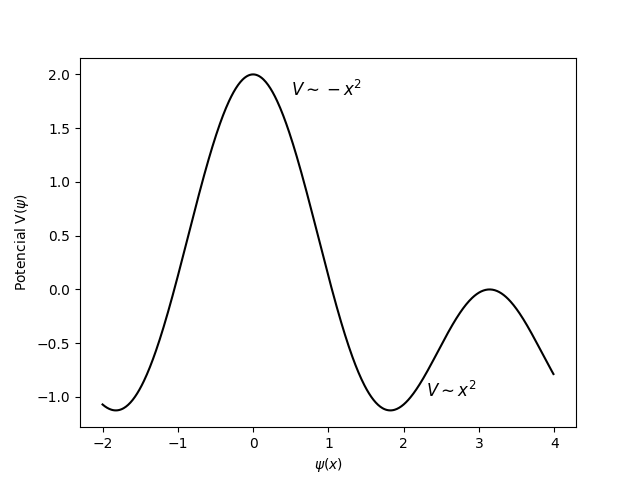
\includegraphics[width=0.8\columnwidth]{potencial.png}
\caption{ Posible potencial localmente de la forma $V \sim -m^2 \psi^2(x)$. Nótese que se está estudiando el problema en un punto crítico altamente inestable que tenderá a decaer al minimo global que tendrá una forma $V \sim m^2 \psi^2(x)$. }
\label{fig:potencial}
\end{figure}
 
 Si consideramos un campo taquiónico escalar con una masa compleja $\psi(x)$ y le asociamos un potencial escalar localmente como $V \sim m^2 \psi^2(x) $ notamos que estamos en un punto máximo de energía, pues $m^2<0$ y tendremos un comportamiento parabólico hacia abajo (ver figura \ref{fig:potencial}), así que el potencial adquiere un valor máximo. Un campo taquiónico es completamente inestable cerca del máximo local del potencial así que evoluciona a una masa cuadrada no negativa y se vuelve estable cerca del mínimo \cite{copeland2005needed}. En otras palabras, el potencial del campo nos revela que se está estudiando el campo taquiónico en un máximo de energía potencial que es un punto inestable, y esto quiere decir que el campo es inestable, lo cual es en muchos casos de la física, un error y se debe buscar un punto donde la energía sea mínima. Sin embargo en el punto donde la energía es mínima corresponderá a una parábola hacia arriba que se podrá aporximar con una masa cuadrada positiva y allí no existen partículas taquiónicas. Es por esto que es natural pensar que ocurrirá un condensado de partículas por el carácter inestable del campo.

La aparición de taquiones es un problema potencialmente grave para cualquier teoría. Los ejemplos de campos taquiónicos susceptibles de condensación son todos casos de ruptura espontánea de simetría. En la física de la materia condensada, un ejemplo notable es el ferromagnetismo; en física de partículas, el ejemplo más conocido es el campo de Higgs en el modelo estándar que rompe la simetría electrodébil \cite{kostelecky1988static}.   


\section{Conclusiones}
A pesar de que el campo taquiónico tiene propiedades nunca antes vistas fascinantes a los ojos de la física de partículas, es complicado pensar en su existencia con las teorías válidas actuales ya que los campos no obedecen reglas fundamentales como la invarianza de Lorentz y se podría complicar aún más al darle la interpretación de viajar hacia atrás en el tiempo, pues si este fuera el caso, lo más probable es que habría una ruptura en la causalidad.  

Por otro lado, mientras una hipótesis no pueda ser probada experimentalmente la comunidad científica la observará con escepticismo, y por el hecho de que actualmente no haya manera de detectar los taquiones la partícula es funcional únicamente como partícula virtual.   

Lo más cercano a las aplicaciones del taquión ha sido la hipotética radiación de Cherenkov y el condensado taquiónico, sin embargo la radiación no ha sido medida experimentalmente y el campo taquiónico no dice nada sobre partículas que se mueven a velocidades mayores que $c$, sino que nos habla de su carácter inestable y un posible error teórico al hacer el análisis en un máximo de energía potencial.   



\section{Agradecimientos}

Agradezco principalmente a la Universidad de Antioquia por brindar todas las herramientas necesarias para garantizar la continuación de la mayoría de los estudiantes pese a la contingencia mundial por el virus.
El semestre pasado se complicó bastante encontrar un profesor con buenas dinámicas de enseñanza para la virtualidad, en este hubieron varias excepciones. Por eso finalmente quiero agradecer al profesor Diego por el espacio de alimentación académica y discusión, además de la buena pedagogía en el curso actual.


\bibliography{apssamp} %Esto toma la bibliografía del archivo apssamp.bib y la organiza de manera automática.
\end{document}

